\documentclass[12pt]{article}

\usepackage{graphicx}
\usepackage{amsmath}
\usepackage{amsfonts}
\usepackage{amssymb}
\usepackage{subcaption}
\usepackage{pdfpages}

\def\td{\mathbf{t}}   % response-threshold value

\begin{document}
\includepdf[pages={-}]{nature-text.pdf}

\newpage
\subsection*{Figures}
\begin{figure*}[ht!]
    \centering\begin{subfigure}[t]{0.41\textwidth}
        \centering
        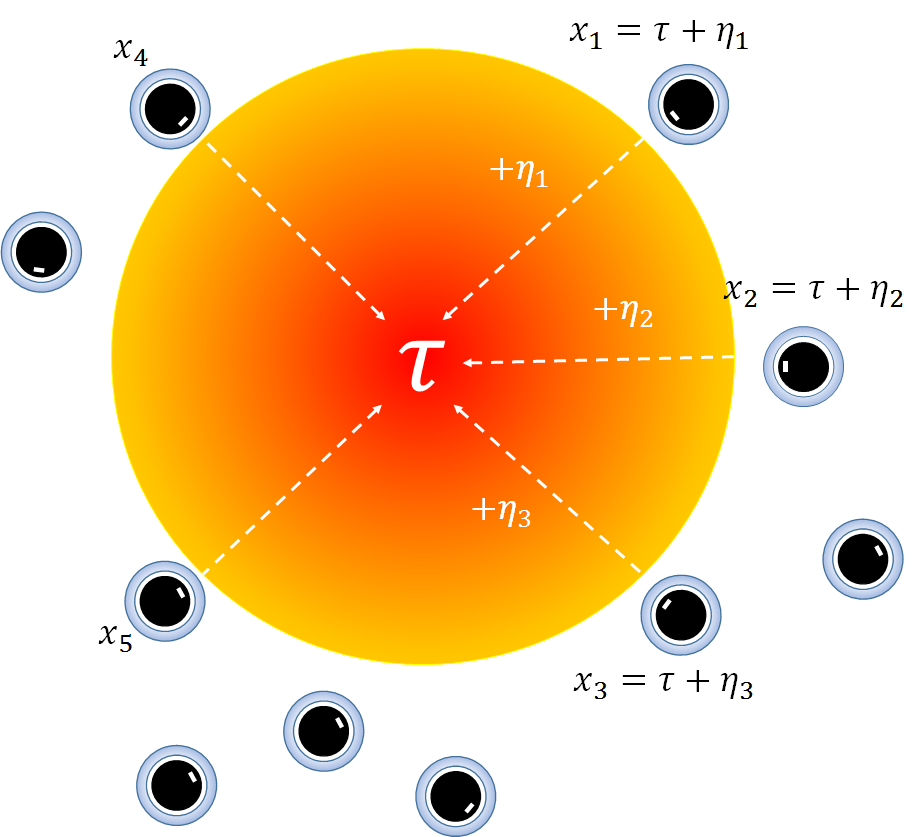
\includegraphics[width=1\textwidth]{figures/firefighting.png}
        \caption{Robot Firefighting}
    \end{subfigure}%
    ~ 
    \begin{subfigure}[t]{0.41\textwidth}
        \centering
        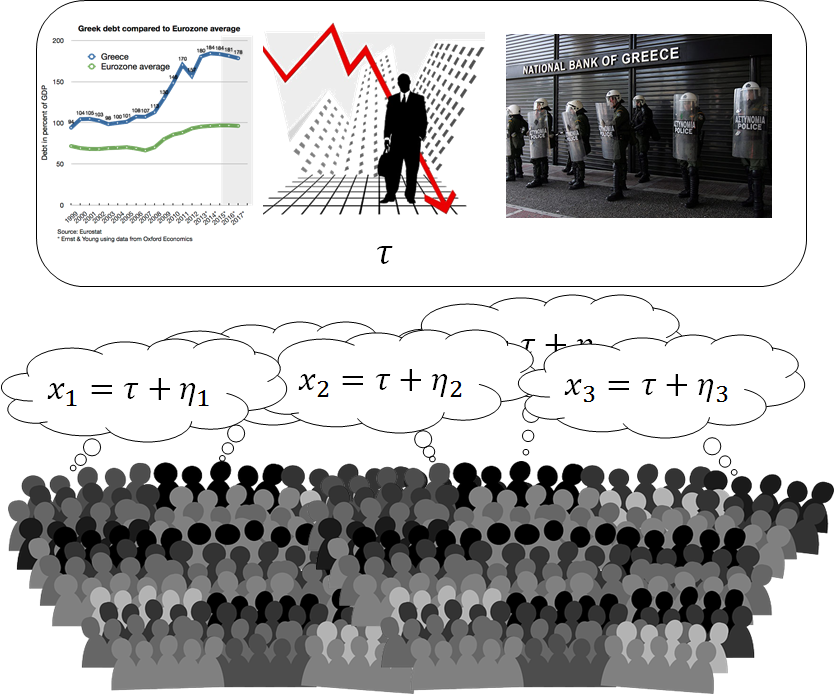
\includegraphics[width=1\textwidth]{figures/bankrun.png}
        \caption{Bank Run}
    \end{subfigure}
    \begin{subfigure}[t]{.82\textwidth}
        \centering
        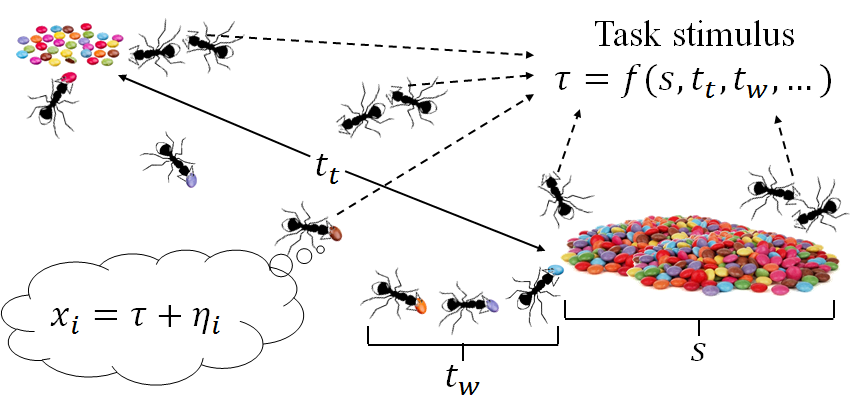
\includegraphics[width=1\textwidth]{figures/foraging.png}
        \caption{Ant Foraging}
    \end{subfigure}    
    \caption{Robotic fire fighting, ant foraging, and bank run scenarios presented as global games. Each player's imperfect estimate of the task is represented by $x_i$, comprising of the global stimulus parameter $\tau$ and noisy sensor measurements $\eta_i$. In the robot firefighting scenario $\tau$ is representative of the magnitude of the fire, while in the case of a bank run $\tau$ is indicative of an agent's current level of trust in the nation's economy. For the ant foraging scenario $\tau$ represents an ant's willingness to take part in the foraging task based on a number of internally measured parameters such as the distance to the food source ($t_t$), the wait time to deliver food ($t_w$), and the food stores currently at the nest ($s$), among others.}    
\end{figure*}

\newpage
\begin{figure}[!ht]
	\centering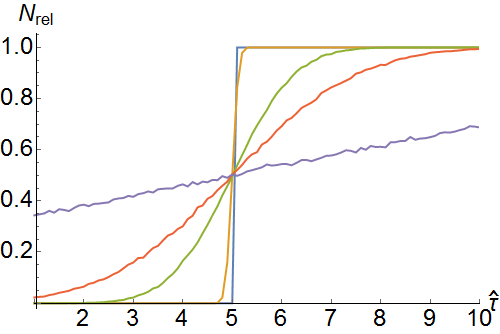
\includegraphics[width=0.7\columnwidth]{figures/thm2fig.png}
	\centering\caption{Visualization of Theorem~2 as $N_{rel}$ estimates $\Phi(\cdot)$. The plot was generated by running Eqn.~1 10,000 times for each point in $\hat{\tau} = 1$ to $10$ in increments of $0.1$. $n = 10$, $\td = 5$ and $x_i = \hat{\tau} + \eta_i$ ($\eta_i \sim\mathcal{N}(0, \sigma^2)$). Each curve in the plot is generated by sweeping $\sigma^2 = \{0, 0.1, 1, 2, 10\}$, with $\sigma^2 = 0$ being a step-function and $\sigma^2 = 10$ having the \emph{flattest} slope.}\label{fig:thm2fig}
\end{figure}
\end{document}